
%-----------------------------------------------------------------------------
% PACKAGES AND OTHER DOCUMENT CONFIGURATIONS
%-----------------------------------------------------------------------------

\documentclass[11pt]{article}
\usepackage[margin=1in]{geometry}
\usepackage{amsmath, amsfonts}
\usepackage{enumerate}
\usepackage{graphicx}
\graphicspath{ {./images/} }
\usepackage{titling}
\usepackage{url}
\usepackage{xfrac}
\usepackage{fancyhdr}
\usepackage{geometry}
\usepackage{graphicx}
\usepackage{natbib}
\usepackage{amsmath}
\usepackage{amssymb}
\usepackage{amsthm}
\usepackage{paralist}
\usepackage{epstopdf}
\usepackage{tabularx}
\usepackage{longtable}
\usepackage{multirow}
\usepackage{multicol}
\usepackage[colorlinks=true,urlcolor=blue]{hyperref}
\usepackage{fancyvrb}
\usepackage{algorithm}
\usepackage{algorithmic}
\usepackage{float}
\usepackage{paralist}
\usepackage[svgname]{xcolor}
\usepackage{enumerate}
\usepackage{array}
\usepackage{times}
\usepackage{url}
\usepackage{fancyhdr}
\usepackage{comment}
\usepackage{environ}
\usepackage{times}
\usepackage{textcomp}
\usepackage{caption}
\usepackage[colorlinks=true,urlcolor=blue]{hyperref}
\usepackage{listings}
\usepackage{parskip} % For NIPS style paragraphs.
\usepackage[compact]{titlesec} % Less whitespace around titles
\usepackage[inline]{enumitem} % For inline enumerate* and itemize*
\usepackage{datetime}
\usepackage{comment}
% \usepackage{minted}
\usepackage{lastpage}
\usepackage{color}
\usepackage{xcolor}
\usepackage{listings}
\usepackage{tikz}
\usetikzlibrary{shapes,decorations}
\usepackage{framed}
\usepackage{booktabs}
\usepackage{cprotect}
\usepackage{fancyvrb}
\usepackage{xcolor}
\usepackage{verbatimbox}
\usepackage[many]{tcolorbox}
\usepackage{cancel}


\newcommand{\blackcircle}{\tikz\draw[black,fill=black] (0,0) circle (1ex);}
\renewcommand{\circle}{\tikz\draw[black] (0,0) circle (1ex);}
\newtcolorbox[]{solution}[1][]{%
    breakable,
    enhanced,
    colback=white,
    title=Solution,
    #1
}

%%%%%%%%%%%%%%%%%%%%%%%%%%%%%%%%%%%%%%%%%%%
% Better numbering                        %
%%%%%%%%%%%%%%%%%%%%%%%%%%%%%%%%%%%%%%%%%%%

\numberwithin{equation}{section} % Number equations within sections (i.e. 1.1, 1.2, 2.1, 2.2 instead of 1, 2, 3, 4)
\numberwithin{figure}{section} % Number figures within sections (i.e. 1.1, 1.2, 2.1, 2.2 instead of 1, 2, 3, 4)
\numberwithin{table}{section} % Number tables within sections (i.e. 1.1, 1.2, 2.1, 2.2 instead of 1, 2, 3, 4)

%%%%%%%%%%%%%%%%%%%%%%%%%%%%%%%%%%%%%%%%%%%
% Code highlighting with listings         %
%%%%%%%%%%%%%%%%%%%%%%%%%%%%%%%%%%%%%%%%%%%

\definecolor{bluekeywords}{rgb}{0.13,0.13,1}
\definecolor{greencomments}{rgb}{0,0.5,0}
\definecolor{redstrings}{rgb}{0.9,0,0}
\definecolor{light-gray}{gray}{0.95}

\newcommand{\MYhref}[3][blue]{\href{#2}{\color{#1}{#3}}}%

\definecolor{dkgreen}{rgb}{0,0.6,0}
\definecolor{gray}{rgb}{0.5,0.5,0.5}
\definecolor{mauve}{rgb}{0.58,0,0.82}

\lstdefinelanguage{Shell}{
  keywords={tar, cd, make},
  %keywordstyle=\color{bluekeywords}\bfseries,
  alsoletter={+},
  ndkeywords={python, py, javac, java, gcc, c, g++, cpp, .txt, octave, m, .tar},
  %ndkeywordstyle=\color{bluekeywords}\bfseries,
  identifierstyle=\color{black},
  sensitive=false,
  comment=[l]{//},
  morecomment=[s]{/*}{*/},
  commentstyle=\color{purple}\ttfamily,
  stringstyle=\color{red}\ttfamily,
  morestring=[b]',
  morestring=[b]",
  backgroundcolor = \color{light-gray}
}

\lstset{columns=fixed, basicstyle=\ttfamily,
    backgroundcolor=\color{light-gray},breaklines=true, xleftmargin=0.5cm,frame=tlbr,framesep=4pt,framerule=0pt}


%%%%%%%%%%%%%%%%%%%%%%%%%%%%%%%%%%%%%%%%%%%
% Custom box for highlights               %
%%%%%%%%%%%%%%%%%%%%%%%%%%%%%%%%%%%%%%%%%%%

% Define box and box title style
\tikzstyle{mybox} = [fill=blue!10, very thick,
    rectangle, rounded corners, inner sep=1em, inner ysep=1em]

% \newcommand{\notebox}[1]{
% \begin{tikzpicture}
% \node [mybox] (box){%
%     \begin{minipage}{\textwidth}
%     #1
%     \end{minipage}
% };
% \end{tikzpicture}%
% }

\NewEnviron{notebox}{
\begin{tikzpicture}
\node [mybox] (box){
    \begin{minipage}{\textwidth}
        \BODY
    \end{minipage}
};
\end{tikzpicture}
}

%%%%%%%%%%%%%%%%%%%%%%%%%%%%%%%%%%%%%%%%%%%
% Commands for customizing the assignment %
%%%%%%%%%%%%%%%%%%%%%%%%%%%%%%%%%%%%%%%%%%%

\newcommand{\courseName}{10-301/10-601 Introduction to Machine Learning (Fall 2019)}
\newcommand{\hwName}{Homework 2: Decision Trees}
\newcommand{\outDate}{Wednesday, Sept. 04, 2019}
\newcommand{\dueDate}{Wednesday, Sept. 18, 2019, 11:59 PM}

\pagestyle{fancyplain}
\lhead{\fancyplain{}{\hwName}}
\rhead{\fancyplain{}{\courseName}}
\cfoot{\thepage}

\title{\textsc{\hwName}} % Title


\author{\courseName\\
  Carnegie Mellon University \\
\url{piazza.com/cmu/fall2019/1030110601} \\
OUT: \outDate{}\thanks{Compiled on \today{} at \currenttime{}} \\
DUE: \dueDate{} \\ 
TAs: Sankalp Patro, Kelly Shi, Yue Yin, Eric Chen}

\date{}

%%%%%%%%%%%%%%%%%%%%%%%%%%%%%%%%%%%%%%%%%%%%%%%%%
% Useful commands for typesetting the questions %
%%%%%%%%%%%%%%%%%%%%%%%%%%%%%%%%%%%%%%%%%%%%%%%%%

\newcommand \expect {\mathbb{E}}
\newcommand \mle [1]{{\hat #1}^{\rm MLE}}
\newcommand \map [1]{{\hat #1}^{\rm MAP}}
\newcommand \argmax {\operatorname*{argmax}}
\newcommand \argmin {\operatorname*{argmin}}
\newcommand \code [1]{{\tt #1}}
\newcommand \datacount [1]{\#\{#1\}}
\newcommand \ind [1]{\mathbb{I}\{#1\}}

%%%%%%%%%%%%%%%%%%%%%%%%%%
% Document configuration %
%%%%%%%%%%%%%%%%%%%%%%%%%%

% Don't display a date in the title and remove the white space
\predate{}
\postdate{}
\date{}

% Don't display an author and remove the white space
%\preauthor{}
%\postauthor{}

%%%%%%%%%%%%%%%%%%
% Begin Document %
%%%%%%%%%%%%%%%%%% 

\begin{document}

\maketitle

\begin{notebox}
\paragraph{Summary} It's time to build your first end-to-end learning system! In this assignment, you will build a Decision Tree classifier and apply it to several binary classification problems. This assignment consists of several parts: In Section \ref{sec:warmup}, you will work through some Information Theory basics in order to ``learn'' a Decision Tree on paper. Then in Section \ref{sec:programming}, you will implement Decision Tree learning, prediction, and evaluation. Using that implementation, you will answer a few empirical questions in Section \ref{sec:empirical}
\end{notebox}

\section*{START HERE: Instructions}
\begin{itemize}

\item \textbf{Collaboration Policy}: Collaboration on solving the homework is allowed, after you have thought about the problems on your own. It is also OK to get clarification (but not solutions) from books or online resources, again after you have thought about the problems on your own. There are two requirements: first, cite your collaborators fully and completely (e.g., ``Jane explained to me what is asked in Question 3.4''). Second, write your solution {\em independently}: close the book and all of your notes, and send collaborators out of the room, so that the solution comes from you only.  See the collaboration policy on the website for more information: \url{http://www.cs.cmu.edu/~mgormley/courses/10601/about.html}
\item\textbf{Late Submission Policy:} See the late submission policy
  here:
  \url{http://www.cs.cmu.edu/~mgormley/courses/10601/about.html}

\item\textbf{Submitting your work:} You will use Gradescope to submit
  answers to all questions, and Autolab to submit your code. Please
  follow instructions at the end of this PDF to correctly submit all your code to Autolab.

  \begin{itemize}
    
  % COMMENT IF NOT USING CANVAS
\begin{comment}
  \item \textbf{Canvas:} Canvas (\url{https://canvas.cmu.edu}) will be
    used for quiz-style problems (e.g. multiple choice, true / false,
    numerical answers). Grading is done automatically.
    %
    You may only \textbf{submit once} on canvas, so be sure of your
    answers before you submit. However, canvas allows you to work on
    your answers and then close out of the page and it will save your
    progress.  You will not be granted additional submissions, so
    please be confident of your solutions when you are submitting your
    assignment.
    %
    {\color{red} The above is true for future assignments, but this one
    allows {\bf unlimited submissions}.}
\end{comment}
    
  % COMMENT IF NOT USING GRADESCOPE
   \item \textbf{Gradescope:} For written problems such as derivations,
       proofs, or plots we will be using Gradescope
       (\url{https://gradescope.com/}). Submissions can be handwritten, but
       should be labeled and clearly legible. If your writing is not
       legible, you will not be awarded marks. Alternatively, submissions
       can be written in LaTeX. Upon submission, label each question
       using the template provided. Regrade requests can be made, however
       this gives the TA the opportunity to regrade your entire paper,
       meaning if additional mistakes are found then points will be
       deducted.
       %   
       Each derivation/proof should be  completed on a separate page.

  %   COMMENT IF NOT USING AUTOLAB
  \item \textbf{Autolab:} You will submit your code for programming
    questions on the homework to Autolab
    (\url{https://autolab.andrew.cmu.edu/}). After uploading your code,
    our grading scripts will autograde your assignment by running your
    program on a virtual machine (VM). 
    %
    The software installed on the VM is identical to that on
    \texttt{linux.andrew.cmu.edu}, so you should check that your code
    runs correctly there. If developing locally, check that the
    version number of the programming language environment
    (e.g. Python 2.7/3.5, Octave 3.8.2, OpenJDK 1.8.0, g++ 4.8.5) and
    versions of permitted libraries (e.g. \texttt{numpy} 1.7.1 and \texttt{scipy} 0.12.1 for Python 2.7 and \texttt{numpy} 1.14.1 and \texttt{scipy} 1.0.1 for Python 3.5) 
    match those on \texttt{linux.andrew.cmu.edu}. DO NOT use any 3rd party
    python packages (i.e. \texttt{sklearn} or \texttt{pandas}) in your implementation! 
    Note: Also do not use \texttt {numpy.loadtxt()}.
    % 
    (Octave users: Please make sure you do not use any
    Matlab-specific libraries in your code that might make it fail
    against our tests.)
    %
    You have a {\bf total of 10 Autolab submissions}. Use them
    wisely. In order to not waste Autolab submissions, we recommend
    debugging your implementation on the linux servers to make sure 
    your code is running correctly first
    before any Autolab submission. 
    %
    
  \end{itemize}

\item\textbf{Materials:} Download from autolab the tar file ("Download
  handout"). The tar file will contain all the data that you will need in order to complete this assignment.

\end{itemize}

For multiple choice or select all that apply questions, shade in the box or circle in the template document corresponding to the correct answer(s) for each of the questions. For \LaTeX users, use $\blacksquare$ and $\blackcircle$  for shaded boxes and circles, and don't change anything else.


\clearpage

\section*{Instructions for Specific Problem Types}

For ``Select One" questions, please fill in the appropriate bubble completely:

\begin{quote}
\textbf{Select One:} Who taught this course?
\begin{list}{}
     \item $\blackcircle$ Matt Gormley
     \item $\circle$ Marie Curie
     \item $\circle$ Noam Chomsky
\end{list}
\end{quote}

If you need to change your answer, you may cross out the previous answer and bubble in the new answer:

\begin{quote}
\textbf{Select One:} Who taught this course?
\begin{list}{}
     \item $\blackcircle$ Matt Gormley
     \item $\circle$ Marie Curie\\
     \xcancel{$\blackcircle$}{} Noam Chomsky
\end{list}
\end{quote}


For ``Select all that apply" questions, please fill in all appropriate squares completely:

\begin{quote}
\textbf{Select all that apply:} Which are scientists?
    \begin{list}{}
    \item $\blacksquare$ Stephen Hawking 
    \item $\blacksquare$ Albert Einstein
    \item $\blacksquare$ Isaac Newton
    \item $\square$ I don't know
\end{list}
\end{quote}

Again, if you need to change your answer, you may cross out the previous answer(s) and bubble in the new answer(s):

\begin{quote}
\textbf{Select all that apply:} Which are scientists?
    \begin{list}{}
    \item $\blacksquare$ Stephen Hawking 
    \item $\blacksquare$ Albert Einstein
    \item $\blacksquare$ Isaac Newton\\
    \xcancel{$\blacksquare$} I don't know
\end{list}
\end{quote}

For questions where you must fill in a blank, please make sure your final answer is fully included in the given space. You may cross out answers or parts of answers, but the final answer must still be within the given space.

\begin{quote}
\textbf{Fill in the blank:} What is the course number?

\begin{tcolorbox}[fit,height=1cm, width=4cm, blank, borderline={1pt}{-2pt},nobeforeafter]
    \begin{center}\huge10-601\end{center}
    \end{tcolorbox}\hspace{2cm}
    \begin{tcolorbox}[fit,height=1cm, width=4cm, blank, borderline={1pt}{-2pt},nobeforeafter]
    \begin{center}\huge10-\xcancel{7}601\end{center}
    \end{tcolorbox}
\end{quote}
\clearpage

\section{Written Questions [25pts]}
\label{sec:written}

Answer the following questions in the HW2 solutions template provided. DO NOT show your work. Then upload your solutions to Gradescope.

\subsection{Warm-up}
\label{sec:warmup}

First, let's think a little bit about decision trees. The following dataset consists of 7 examples, each with 3 attributes, $(A,B,C)$, and a label, $Y$.

\begin{center}
\begin{tabular}{|c|c|c|c|}
\hline
$A$ & $B$ & $C$ & $Y$ \\ \hline
1 & 1 & 0 & 0     \\ \hline
1 & 1 & 2 & 1     \\ \hline
1 & 0 & 0 & 1     \\ \hline
1 & 1 & 2 & 1     \\ \hline
0 & 0 & 2 & 0     \\ \hline
0 & 1 & 1 & 0     \\ \hline
0 & 0 & 0 & 0     \\ \hline
\end{tabular}
\end{center}


Use the data above to answer the following questions. 

\begin{notebox}
A few important notes:
\begin{itemize}
    \item \emph{All calculations should be done without rounding!} After you have finished all of your calculations, write your rounded solutions in the boxes below.
    %\item Unless otherwise noted, numeric solutions should include 4 digits of precision (e.g. 0.1234).
    \item Note that, throughout this homework, we will use the convention that the leaves of the trees do not count as nodes, and as such are not included in calculations of depth and number of splits. (For example, a tree which classifies the data based on the value of a single attribute will have depth 1, and contain 1 split.)
\end{itemize}
\end{notebox}

\begin{enumerate}
    \item \textbf{[1pt]} What is the entropy of $Y$ in bits, $H(Y)$? In this and subsequent questions, when we request the units in \emph{bits}, this simply means that you need to use $\log$ base 2 in your calculations.\footnote{If instead you used $\log$ base $e$, the units would be \emph{nats}; $\log$ base 10 gives \emph{bats}.}
    %
    (Please include one number rounded to the fourth decimal place, e.g. 0.1234)
    
    \begin{tcolorbox}[fit,height=1cm, width=2cm, blank, borderline={1pt}{-2pt},nobeforeafter]
    %solution 
    \begin{center}\huge0.9852\end{center}
    \end{tcolorbox}
    
    
    \item \textbf{[1pt]} What is the mutual information\footnote{In the context of decision trees, and therefore in this assignment, the terms ``information gain" and ``mutual information" are synonymous (e.g. they have the same meaning as one another). However, in information theory and machine learning in general, ``information gain" is synonymous with ``Kullback-Leibler (K-L) divergence", often referred to as relative entropy, which is not the same as mutual information. For more information, go \href{https://en.wikipedia.org/wiki/Information_gain_in_decision_trees}{here.} } 
    of $Y$ and $A$ in bits, $I(Y; A)$?
    %
    (Please include one number rounded to the fourth decimal place, e.g. 0.1234)
    
    \begin{tcolorbox}[fit,height=1cm, width=2cm, blank, borderline={1pt}{-2pt},nobeforeafter]
    %solution 
    \begin{center}\huge0.5216\end{center}
    \end{tcolorbox}
    

\clearpage
    \item \textbf{[1pt]} What is the mutual information of $Y$ and $B$ in bits, $I(Y; B)$?
    %
    (Please include one number rounded to the fourth decimal place, e.g. 0.1234)
    
    \begin{tcolorbox}[fit,height=1cm, width=2cm, blank, borderline={1pt}{-2pt},nobeforeafter]
    %solution 
    \begin{center}\huge0.0202\end{center}
    \end{tcolorbox}
    
    
    \item \textbf{[1pt]} What is the mutual information of $Y$ and $C$ in bits, $I(Y; C)$?
    %
    (Please include one number rounded to the fourth decimal place, e.g. 0.1234)
    
    \begin{tcolorbox}[fit,height=1cm, width=2cm, blank, borderline={1pt}{-2pt},nobeforeafter]
    %solution 
    \begin{center}\huge0.1981\end{center}
    \end{tcolorbox}
    
    
    \item \textbf{[1pt]} Consider the dataset given above. Which attribute ($A$, $B$, or $C$) would a decision tree algorithm pick first to branch on, if its splitting criterion is mutual information?
    
    \textbf{Select one:}
    \begin{list}{}
        \item $\blackcircle$ $A$
        \item $\circle$ $B$
        \item $\circle$ $C$
    \end{list}
    
    
    \item \textbf{[1pt]} Consider the dataset given above. Which is the second attribute you would pick to branch on, if its splitting criterion is mutual information? (\emph{Hint:} Notice that this question correctly presupposes that there is \emph{exactly one} second attribute.)
    
    \textbf{Select one:}
    \begin{list}{}
        \item $\circle$ $A$
        \item $\circle$ $B$
        \item $\blackcircle$ $C$
    \end{list}
    
    
    \item \textbf{[1pt]} If the same algorithm continues until the tree perfectly classifies the data, what would the depth of the tree be?
    
    \begin{tcolorbox}[fit,height=1cm, width=2cm, blank, borderline={1pt}{-2pt},nobeforeafter]
    %solution 
    \begin{center}\Huge3\end{center}
    \end{tcolorbox}
    
    
\clearpage
    \item \textbf{[4pt]} Draw your completed Decision Tree. Label the non-leaf nodes with which attribute the tree will split on (e.g. $B$), the edges with the value of the attribute (e.g. 1 or 0), and the leaf nodes with the classification decision (e.g. $Y=0$).
    
    \begin{solution}
    % If you are using the latex template, remove the empty spaces
    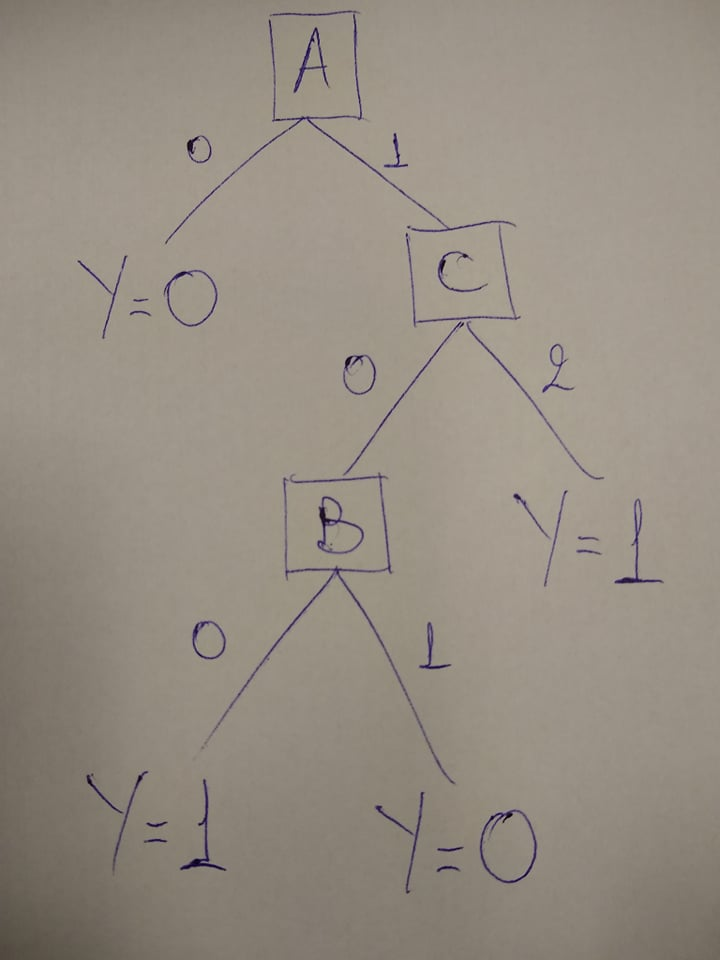
\includegraphics[scale=0.5]{decTree}
  
    \end{solution}
    
\end{enumerate}

\clearpage
\subsection{Empirical Questions}
\label{sec:empirical}

The following questions should be completed as you work through the programming portion of this assignment (Section \ref{sec:programming}).

 \begin{enumerate}
    \item[9.] \textbf{[2pt]} Train and test your decision tree on the politician dataset and the education dataset with four different values of max-depth, $\{0,1,2,4\}$. Report your findings in the HW2 solutions template provided. A Decision Tree with max-depth 0 is simply a \emph{majority vote classifier}; a Decision Tree with max-depth 1 is called a \emph{decision stump}. If desired, you could even check that your answers for these two simple cases are correct using your favorite spreadsheet application (e.g. Excel, Google Sheets). (Please round each number to the fourth decimal place, e.g. 0.1234)
    
    \begin{center}
    \begin{tabular}{cc|c|c}
        \toprule
      {\bf Dataset}   & {\bf Max-Depth} & {\bf Train Error} & {\bf Test Error} \\
      \midrule
        politician & 0 & 0.4429 & 0.5060\\
        politician & 1 & 0.2013 & 0.2169\\
        politician & 2 & 0.1342 & 0.1566\\
        politician & 4 & 0.1074 & 0.1807\\
        \midrule
        education & 0 & 0.3250 & 0.3100\\
        education & 1 & 0.1950 & 0.2300\\
        education & 2 & 0.1950 & 0.2300\\
        education & 4 & 0.1300 & 0.1600\\
        \bottomrule
    \end{tabular}
    \end{center}
    
    
    \item[10.] \textbf{[3pt]} For the politicians dataset, create a computer-generated plot showing error on the y-axis against depth of the tree on the x-axis. Plot \emph{both} training error and testing error, clearly labeling which is which.  That is, for each possible value of max-depth ($0, 1, 2, \ldots,$ up to the number of attributes in the dataset), you should train a decision tree and report train/test error of the model's predictions.
    
    \begin{solution}
    % If you are using the latex template, remove the empty spaces
    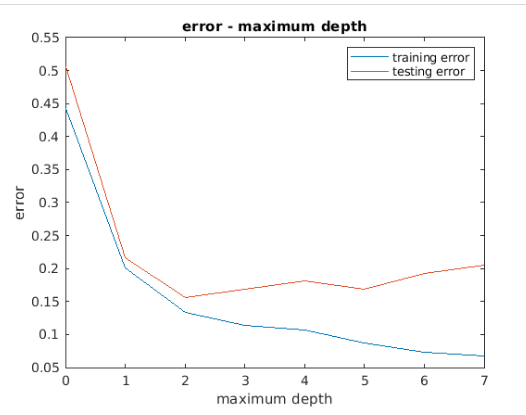
\includegraphics[scale=0.5]{plot}
    \end{solution}
    
\clearpage
    \item[11.] \textbf{[2pt]} Suppose your research advisor asks you to run some model selection experiments and then report your results. You select the Decision Tree model's max-depth to be the one with lowest test error in metrics.txt and then report that model's test error as the performance of our classifier on held out test data. Is this a good experimental setup? If so, why? If not, why not?
    
    \begin{solution}
    % If you are using the latex template, remove the empty spaces
	No, this is not a good setup. The fact that the implemented algorithm gave us the smallest error with a specific value of maximum depth on the dataset we tested on does not mean that for any unseen (held out) dataset, our algorithm is also going to give us an error of the same scale. So, generalizing and claiming that our algorithm has a good accuracy for any given dataset, based on our test results makes our model biased and should not be done. There is a chance that if we test our algorithm with a large amount of unseen data, the error could be much larger, thus our claim for the performance of our algorithm would be proven entirely wrong.
    \end{solution}
    

    \item[12.] \textbf{[2pt]} In this assignment, we used max-depth as our stopping criterion, and as a mechanism to prevent overfitting. Alternatively, we could stop splitting a node whenever the mutual information for the best attribute is lower than a threshold value. This threshold would be another hyperparameter. Theoretically, how would increasing this threshold value affect the number of nodes and depth of the learned trees?
    
    \begin{solution}
    % If you are using the latex template, remove the empty spaces
    An increase to the threshold value will decrease both the number of nodes and the depth of the tree. That is because, after a point, nodes with attributes that correspond to a lower information gain would not grow further, and this would, in a sense, prune our tree before we even grew it.
    \end{solution}
    

\clearpage
    \item[13.] \textbf{[2pt]} From question 12, how would you set-up model training to choose the threshold value?
    
    \begin{solution}
    % If you are using the latex template, remove the empty spaces
	I believe that a good method would be to start from a big threshold and gradually decrease it. At each iteration we should observe the training and testing error. When we see a behavior that we deem acceptable, we should stop. For example, if we see that the testing error starts to increase after a certain threshold, we should stop, since that would signal that our algorithm is beginning to overfit our data.
    \end{solution}
    
    
\clearpage
    \item[14.] \textbf{[3pt]} Print (do not handwrite!) the decision tree which is produced by your algorithm for the politician data with max depth 3. Instructions on how to print the tree could be found in section \ref{sec:printtree}.
    
     \begin{solution}
    % If you are using the latex template, remove the empty spaces
     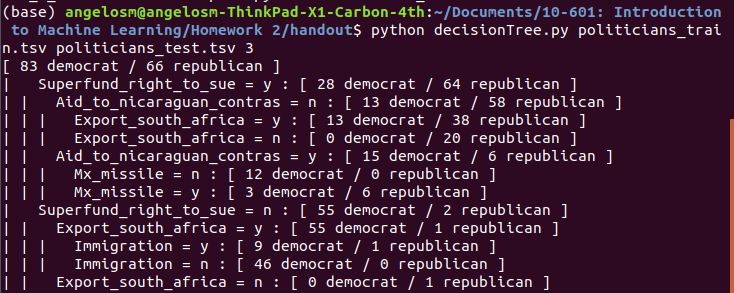
\includegraphics[scale=0.5]{politicians}
    \end{solution}



    
    
    \clearpage
    \item[15.] After you have completed all other components of this assignment, report your answers to the collaboration policy questions detailed in the Academic Integrity Policies found \href{http://www.cs.cmu.edu/~mgormley/courses/10601bd-f18/about.html#7-academic-integrity-policies}{here}.
    \begin{enumerate*}
        \item Did you receive any help whatsoever from anyone in solving this assignment? Is so, include full details.
        \item Did you give any help whatsoever to anyone in solving this assignment? Is so, include full details.
        \item Did you find or come across code that implements any part of this assignment ? If so, include full details.
    \end{enumerate*}
    
    \begin{solution}
    % If you are using the latex template, remove the empty spaces
    No, I did not: a) receive any help from anyone, b) give any help to anyone or c) find any code that implements any part of this assignment.
 
    \end{solution}
    
\end{enumerate}

\newpage
\section{Programming [75pts]}
\label{sec:programming}

Your goal in this assignment is to implement a binary classifier, entirely from scratch--specifically a Decision Tree learner. In addition, we will ask you to run some end-to-end experiments on two tasks (predicting the party of a politician / predicting final grade for high school students) and report your results.
%
You will write two programs: \texttt{inspect.\{py|java|cpp|m\}} (Section \ref{sec:inspect}) and \texttt{decisionTree.\{py|java|cpp|m\}} (Section \ref{sec:decisiontree}). The programs you write will be automatically graded using the Autolab system. You may write your programs in \textbf{Octave}, \textbf{Python}, \textbf{Java}, or \textbf{C++}. However, you should use the same language for all parts below.

\subsection{The Tasks and Datasets}
\label{sec:data}

\paragraph{Materials} Download the tar file from Autolab (``Download
  handout''). The tar file will contain all the data that you will need
  in order to complete this assignment.

\paragraph{Datasets}

The handout contains three datasets. Each one contains attributes and labels and is already split into training and testing data. The first line of each \lstinline{.tsv} file contains the name of each attribute, and \emph{the class is always the last column}.

\begin{enumerate}
\item \textbf{politician:}
    The first task is to predict whether a US politician is a member of the Democrat or Republican party, based on their past voting history. Attributes (aka. features) are short descriptions of bills that were voted on, such as \emph{Aid\_to\_nicaraguan\_contras} or \emph{Duty\_free\_exports}. Values are given as \emph{`y'} for yes votes and \emph{`n'} for no votes. The training data is in \lstinline{politicians_train.tsv}, and the test data in \lstinline{politicians_test.tsv}.
\item \textbf{education:}
    The second task is to predict the final \emph{grade} (A, not A) for high school students. The attributes (covariates, predictors) are student grades on 5 multiple choice assignments \emph{M1} through \emph{M5}, 4 programming assignments \emph{P1} through \emph{P4}, and the final exam \emph{F}. The training data is in \newline \lstinline{education_train.tsv}, and the test data in \lstinline{education_test.tsv}.
\item \textbf{small:}
    We also include \lstinline{small_train.tsv} and \lstinline{small_test.tsv}---a small, purely for demonstration version of the politicians dataset, with \emph{only} attributes \emph{Anti\_satellite\_test\_ban} and \newline \emph{Export\_south\_africa}.  
    For this small dataset, the handout tar file also contains the predictions from a reference implementation of a Decision Tree with max-depth 3 (see \lstinline{small_3_train.labels}, \lstinline{small_3_test.labels}, \lstinline{small_3_metrics.txt}).
    You can check your own output against these to see if your implementation is correct.\footnote{Yes, you read that correctly: we are giving you the correct answers.}
\end{enumerate}

\begin{notebox} \textbf{Note:}
For simplicity, all attributes are discretized into just two categories (i.e. each node will have at most two descendents). This applies to all the datasets in the handout, as well as the additional datasets on which we will evaluate your Decision Tree.
\end{notebox}

\newpage
\subsection{Program \#1: Inspecting the Data [5pts]}
\label{sec:inspect}

Write a program \texttt{inspect.\{py|java|cpp|m\}} to calculate the label entropy at the root (i.e. the entropy of the labels before any splits) and the error rate (the percent of incorrectly classified instances) of classifying using a majority vote (picking the label with the most examples). You do not need to look at the values of any of the attributes to do these calculations, knowing the labels of each example is sufficient. \textbf{Entropy should be calculated in bits using log base 2.}

\paragraph{Command Line Arguments}
The autograder runs and evaluates the output from the files  generated, using the following command:

\begin{tabular}{ll}
 For Python:
 &
\begin{lstlisting}[language=Shell]
$ python inspect.py <input> <output>
\end{lstlisting}
\\
For Java:
&
\begin{lstlisting}[language=Shell]
$ javac inspect.java; java inspect <input> <output>
\end{lstlisting}
\\
% For C:
% \begin{lstlisting}[language=Shell]
% $ gcc inspect.c; ./a.out <input> <output>
% \end{lstlisting}
For C++:
&
\begin{lstlisting}[language=Shell]
$ g++ inspect.cpp; ./a.out <input> <output>
\end{lstlisting}
\\
For Octave:
&
\begin{lstlisting}[language=Shell]
$ octave -qH inspect.m <input> <output>
\end{lstlisting}
\\
\end{tabular}

Your program should accept two command line arguments: an input file and an output file. It should read the \lstinline{.tsv} input file (of the format described in Section \ref{sec:data}), compute the quantities above, and write them to the output file so that it contains:
\begin{quote}
\begin{verbatim}
entropy: <entropy value>
error: <error value>
\end{verbatim}
\end{quote}

\paragraph{Example}

For example, suppose you wanted to inspect the file \lstinline{small_train.tsv} and write out the results to \lstinline{small_inspect.txt}. For Python, you would run the command below:
%
\begin{lstlisting}[language=Shell]
$ python inspect.py small_train.tsv small_inspect.txt
\end{lstlisting}
%
Afterwards, your output file \lstinline{small_inspect.txt} should contain the following:
%
\begin{quote}
\begin{verbatim}
entropy: 0.996316519559
error: 0.464285714286
\end{verbatim}
\end{quote}
%
Our autograder will run your program on several input datasets to check that it correctly computes entropy and error, and will take minor differences due to rounding into account. You do not need to round your reported numbers! The Autograder will automatically incorporate the right tolerance for float comparisons.

\begin{notebox}
For your own records, run your program on each of the datasets provided in the handout---this error rate for a \emph{majority vote} classifier is a baseline over which we would (ideally) like to improve.
\end{notebox}

\newpage
\subsection{Program \#2: Decision Tree Learner [75pts]}
\label{sec:decisiontree}

In decisionTree.\{py $\mid$ java $\mid$ cpp $\mid$ m\}, implement a Decision Tree learner. This file should learn a decision tree with a specified maximum depth, print the decision tree in a specified format, predict the labels of the training and testing examples, and calculate training and testing errors.

Your implementation must satisfy the following requirements:
\begin{itemize}
\item Use mutual information to determine which attribute to split on.
\item Be sure you're correctly weighting your calculation of mutual information. For a split on attribute X, $I(Y;X)=H(Y)-H(Y|X)=H(Y)-P(X =0)H(Y|X =0)-P(X =1)H(Y|X =1)$.  Equivalently, you can calculate $I (Y ; X ) = H (Y ) + H (X ) - H (Y , X )$.
\item As a stopping rule, only split on an attribute if the mutual information is $>$ 0.
\item Do not grow the tree beyond a max-depth specified on the command line. For example, for a maximum depth of 3, split a node only if the mutual information is $>$ 0 and the current level of the node is $< 3$.
\item Use a majority vote of the labels at each leaf to make classification decisions. If the vote is tied, any classification of the leaf is considered to be correct (all one class, all the other class, or any split of classes).
\item Do not hard-code any aspects of the datasets into your code. We will autograde your programs on two (hidden) datasets that include different attributes and output labels.
\end{itemize}

Careful planning will help you to correctly and concisely implement your Decision Tree learner. Here are a few \emph{hints} to get you started:
\begin{itemize}
    \item Write helper functions to calculate entropy and mutual information.
    \item Write a function to train a stump (tree with only one level). Then call that function recursively to create the sub-trees.
    \item In the recursion, keep track of the depth of the current tree so you can stop growing the tree beyond the max-depth.
    \item Implement a function that takes a learned decision tree and data as inputs, and generates predicted labels. You can write a separate function to calculate the error of the predicted labels with respect to the given (ground-truth) labels.
    \item Be sure to correctly handle the case where the specified maximum depth is greater than the total number of attributes.
    \item Be sure to handle the case where max-depth is zero (i.e. a majority vote classifier). 
    \item Look under the FAQ's on Piazza for more useful clarifications about the assignment.
\end{itemize}

\subsubsection{Command Line Arguments}
%The correct tree and output format for the example data are shown below, where we are training on example1.tsv and testing on example2.tsv. For the politician data, use \textbf{``democrat"} for Party = ``democrat" and \textbf{``republican"} for Party = ``republican". With the education data, use \textbf{``A"} for final grade = ``A" and \textbf{``not A"} for final grade = ``not A". The order in which you list the left and right children does not matter when printing the tree. Your program should be named decisionTree and take three arguments, a training file, a test file, and an integer argument for maximum depth of the tree that should be generated.

The autograder runs and evaluates the output from the files  generated, using the following command:

\begin{tabular}{ll}
For Python: &
\begin{lstlisting}[language=Shell]
$ python decisionTree.py [args...]
\end{lstlisting}
\\
For Java: &
\begin{lstlisting}[language=Shell]
$ javac decisionTree.java; java decisionTree [args...]
\end{lstlisting}
\\
For C++: &
\begin{lstlisting}[language=Shell]
$ g++ decisionTree.cpp; ./a.out [args...]
\end{lstlisting}
\\
For Octave: &
\begin{lstlisting}[language=Shell]
$ octave -qH decisionTree.m [args...]
\end{lstlisting}
\end{tabular}


% \begin{tabbing}
% For Python: \= 
% \lstinline[language=Shell]{$ python decisionTree.py [args...]} \\
% For Java: \> 
% \lstinline[language=Shell]{$ javac decisionTree.java; java decisionTree [args...]}}\\
% For C++: \> 
% \lstinline[language=Shell]{$ g++ decisionTree.cpp; ./a.out [args...]} \\
% For Octave: \> 
% \lstinline[language=Shell]{$ octave -qH decisionTree.m [args...]}
% \end{tabbing}

Where above \lstinline{[args...]} is a placeholder for six command-line arguments: 
\texttt{<train input> <test input> <max depth> <train out> <test out> <metrics out>}. These arguments are described in detail below:
\begin{enumerate}
\item \lstinline{<train input>}: path to the training input \lstinline{.tsv} file (see Section \ref{sec:data})
\item \lstinline{<test input>}: path to the test input \lstinline{.tsv} file (see Section \ref{sec:data})
\item \lstinline{<max depth>}: maximum depth to which the tree should be built
\item \lstinline{<train out>}: path of output \lstinline{.labels} file to which the predictions on the \textit{training} data should be written (see Section \ref{sec:labels})
\item \lstinline{<test out>}: path of output \lstinline{.labels} file to which the predictions on the \emph{test} data should be written (see Section \ref{sec:labels})
\item \lstinline{<metrics out>}: path of the output \lstinline{.txt} file to which metrics such as train and test error should be written (see Section \ref{sec:metrics})
\end{enumerate}

As an example, if you implemented your program in Python, the following command line would run your program on the politicians dataset and learn a tree with max-depth of two. The train predictions would be written to \lstinline{pol_2_train.labels}, the test predictions to \lstinline{pol_2_test.labels}, and the metrics to \lstinline{pol_2_metrics.txt}.
%
\begin{lstlisting}[language=Shell]
$ python decisionTree.py politicians_train.tsv politicians_test.tsv \ 
        2 pol_2_train.labels pol_2_test.labels pol_2_metrics.txt
\end{lstlisting}
%
The following example would run the same learning setup except with max-depth three, and conveniently writing to analogously named output files, so you can can compare the two runs.
%
\begin{lstlisting}[language=Shell]
$ python decisionTree.py politicians_train.tsv politicians_test.tsv \ 
        3 pol_3_train.labels pol_3_test.labels pol_3_metrics.txt
\end{lstlisting}

\subsubsection{Output: Labels Files}
\label{sec:labels}

Your program should write two output \lstinline{.labels} files containing the predictions of your model on training data (\lstinline{<train out>}) and test data (\lstinline{<test out>}). Each should contain the predicted labels for each example printed on a new line. Use '\textbackslash n' to create a new line.

Your labels should exactly match those of a reference decision tree implementation---this will be checked by the autograder by running your program and evaluating your output file against the reference solution.

\textbf{Note}: You should output your predicted labels using the same string identifiers as the original training data: e.g., for the politicians dataset you should output democrat/republican and for the education dataset you should output A/notA.
%
The first few lines of an example output file is given below for the politician dataset:
\begin{quote}
\begin{verbatim}
democrat
democrat
democrat
republican
democrat
...
\end{verbatim}
\end{quote}

\subsubsection{Output: Metrics File}
\label{sec:metrics}

Generate another file where you should report the training error and testing error. This file should be written to the path specified by the command line argument \lstinline{<metrics out>}. Your reported numbers should be within 0.01 of the reference solution. You do not need to round your reported numbers! The Autograder will automatically incorporate the right tolerance for float comparisons. The file should be formatted as follows:

% error(train): 0.3076532
% error(test): 0.4523292
\begin{quote}
\begin{verbatim}
error(train): 0.071429
error(test): 0.142857
\end{verbatim}
\end{quote}

The values above correspond to the results from training a tree of depth 3 on \texttt{small\_train.tsv} and testing on \texttt{small\_test.tsv}.

% \textit{Hint:} Refer to the last section for help on how to save output to a file in different languages.

\subsubsection{Output: Printing the Tree}
\label{sec:printtree}

Finally, you should write a function to pretty-print your learned decision tree. (You may find it more convenient to print the tree \emph{as} you are learning it.) Each row should correspond to a node in the tree. They should be printed in a \emph{depth-first-search} order (but you may print left-to-right or right-to-left). Print the attribute of the node's parent and the attribute value corresponding to the node. Also include the sufficient statistics (i.e. count of positive / negative examples) for the data passed to that node. The row for the root should include \emph{only} those sufficient statistics. A node at depth $d$, should be prefixed by $d$ copies of the string '$\mid$ '.

Below, we have provided the recommended format for printing the tree (example for python). You can print it directly to standard out rather than to a file. \textbf{This functionality of your program will not be autograded}.

\begin{lstlisting}[language=Shell]
$ python decisionTree.py small_train.tsv small_test.tsv 2 \ 
small_2_train.labels small_2_test.labels small_2_metrics.txt

[15 democrat /13 republican]
| Anti_satellite_test_ban = y: [13 democrat /1 republican]
| | Export_south_africa = y: [13 democrat /0 republican]
| | Export_south_africa = n: [0 democrat /1 republican]
| Anti_satellite_test_ban = n: [2 democrat /12 republican]
| | Export_south_africa = y: [2 democrat /7 republican]
| | Export_south_africa = n: [0 democrat /5 republican]
\end{lstlisting}

However, you should be careful that the tree might not be full. For example, after swapping the train/test files in the example above, you could end up with a tree like the following.

\begin{lstlisting}[language=Shell]
$ python decisionTree.py small_test.tsv small_train.tsv 2 \ 
swap_2_train.labels swap_2_test.labels swap_2_metrics.txt

[13 democrat/15 republican]
| Anti_satellite_test_ban = y: [9 democrat/0 republican]
| Anti_satellite_test_ban = n: [4 democrat/15 republican]
| | Export_south_africa = y: [4 democrat/10 republican]
| | Export_south_africa = n: [0 democrat/5 republican]
\end{lstlisting}

The following pretty-print shows the education dataset with max-depth 3.  Use this example to check your code before submitting your pretty-print of the politics dataset (asked in question 14 of the Empirical questions).  

\begin{lstlisting}[language=Shell]
$ python decisionTree.py education_train.tsv education_test.tsv 3 \
edu_3_train.labels edu_3_test.labels edu_3_metrics.txt

[135 A/65 notA]
| F = A: [119 A/23 notA]
| | M4 = A: [56 A/2 notA]
| | | P1 = A: [41 A/0 notA]
| | | P1 = notA: [15 A/2 notA]
| | M4 = notA: [63 A/21 notA]
| | | M2 = A: [37 A/3 notA]
| | | M2 = notA: [26 A/18 notA]
| F = notA: [16 A/42 notA]
| | M2 = A: [13 A/15 notA]
| | | M4 = A: [6 A/1 notA]
| | | M4 = notA: [7 A/14 notA]
| | M2 = notA: [3 A/27 notA]
| | | M4 = A: [3 A/5 notA]
| | | M4 = notA: [0 A/22 notA]
\end{lstlisting}

The numbers in brackets give the number of positive and negative labels from the training data in that part of the tree.

\begin{notebox}
At this point, you should be able to go back and answer questions 9-15 in the "Written Questions" section of this handout.  Write your solutions in the template provided. 
\end{notebox}

\subsubsection{Evaluation}
In addition to the politician and education datasets, Autolab will test your code on two more datasets, which will not be shown to you. One set contains information about various cars, and whether or not consumers decided to buy them. The other contains data about songs, and whether or not they became top hits. The data will be in .tsv files formatted like the ones provided, again with the class as the last column. Shown below are the attributes and the values they can take: 

Music data:

\begin{itemize}
\item \texttt{Attribute:year('before1950'or'after1950')}
\item \texttt{Attribute:solo('yes'or'no')}
\item \texttt{Attribute:vocal('yes'or'no')}
\item \texttt{Attribute:length('morethan3min'or'lessthan3min')}
\item \texttt{Attribute:original('yes'or'no')}
\item \texttt{Attribute:tempo('fast'or'slow')}
\item \texttt{Attribute:folk('yes'or'no')}
\item \texttt{Attribute:classical('yes'or'no')}
\item \texttt{Attribute:rhythm('yes'or'no')}
\item \texttt{Attribute:jazz('yes'or'no')}
\item \texttt{Attribute:rock('yes'or'no')}
\item \texttt{Class Label:hit('yes'or'no')}
\end{itemize}

Cars data:

\begin{itemize}
\item \texttt{Attribute:buying('expensive'or'cheap')}
\item \texttt{Attribute:maint('high'or'low')}
\item \texttt{Attribute:doors('Two'or'MoreThanTwo')}
\item \texttt{Attribute:length('morethan3min'or'lessthan3min')}
\item \texttt{Attribute:person('Two'or'MoreThanTwo')}
\item \texttt{Attribute:boot('large'or'small')}
\item \texttt{Attribute:safety('high'or'low')}
\item \texttt{Class Label:class('yes'or'no')}
\end{itemize}

Please ensure your solution can handle data with these values.

\subsection{Submission Instructions}

\paragraph{Programming}
Please ensure you have completed the following files for submission.

\begin{verbatim}
inspect.{py|java|cpp|m}
decisionTree.{py|java|cpp|m}
\end{verbatim}

When submitting your solution, compress the two files listed above containing your implementation into a tar \lstinline{handin.tar} by running:

\begin{lstlisting}[language=Shell]
$ tar -cvf handin.tar *.{py|java|cpp|m} 
\end{lstlisting}

\textbf{DO NOT} put the above files in a folder and then tar that folder. You must compress the files directly into a  tar file and submit it to Autolab. 
%
\textbf{Note}: Please make sure the programming language that you use is consistent within this assignment (e.g. don't use C++ for inspect and Python for decisionTree).

 \begin{notebox}
  {\bf Python3 Users:} Please include a blank file called python3.txt (case-sensitive) in your tar submission and we will execute your submitted program using Python 3 instead of Python 2.7. If the file is not present, we will default to running your code with Python 2.7.
 \end{notebox} 

\paragraph{Written Questions}
Make sure you have completed all questions from Section \ref{sec:written} (including the collaboration policy questions) in the template provided.  When you have done so, please submit your document in \textbf{pdf format} to the corresponding assignment slot on Gradescope.



\newpage
% \input{saving-to-file.tex}

\end{document}

